%%%%%%%%%%%%%%%%%%%%%%%%%%%%%%%%%%%%%%%%%%%%%%%%%%%%%%%%%%%%%%%%%%%%%%
% Overleaf (WriteLaTeX) Example: Molecular Chemistry Presentation
%
% Source: http://www.overleaf.com
%
% In these slides we show how Overleaf can be used with standard 
% chemistry packages to easily create professional presentations.
% 
% Feel free to distribute this example, but please keep the referral
% to overleaf.com
% 
%%%%%%%%%%%%%%%%%%%%%%%%%%%%%%%%%%%%%%%%%%%%%%%%%%%%%%%%%%%%%%%%%%%%%%

\documentclass{beamer}

\mode<presentation>
{
  \usetheme{Madrid}       % or try default, Darmstadt, Warsaw, ...
  \usecolortheme{default} % or try albatross, beaver, crane, ...
  \usefonttheme{default}    % or try default, structurebold, ...
  \setbeamertemplate{navigation symbols}{}
  \setbeamertemplate{caption}[numbered]
} 

\usepackage[english]{babel}
\usepackage[utf8x]{inputenc}
\usepackage{chemfig}
\usepackage[version=3]{mhchem}

\usepackage{hyperref}
  \hypersetup{colorlinks=true}
  \hypersetup{urlcolor=blue}
  \hypersetup{linkcolor = .}
\usepackage{xcolor}
\usepackage{siunitx}
  \sisetup{separate-uncertainty = true}
\usepackage{physics}
\usepackage[font=small,labelfont=bf]{caption}
\usepackage{subcaption}
\usepackage[en-GB]{datetime2}
\usepackage{overpic}
\usepackage{feynmp}
\DeclareGraphicsRule{*}{mps}{*}{}

\usepackage{scalerel}
\newcommand{\mylbrace}[2]{\vspace{#2pt}\hspace{6pt}\scaleleftright[\dimexpr5pt+#1\dimexpr0.06pt]{\lbrace}{\rule[\dimexpr2pt-#1\dimexpr0.5pt]{-4pt}{#1pt}}{.}}
\newcommand{\myrbrace}[2]{\vspace{#2pt}\scaleleftright[\dimexpr5pt+#1\dimexpr0.06pt]{.}{\rule[\dimexpr2pt-#1\dimexpr0.5pt]{-4pt}{#1pt}}{\rbrace}\hspace{6pt}}

% Here's where the presentation starts, with the info for the title slide
\title[BESIII Oxford]{BESIII Oxford Group Meeting}
\author{Martin Tat}
\institute{Oxford LHCb}
\date{20th May 2021}

\titlegraphic{
\includegraphics[width = 5cm, height = 3.8cm]{lhcb.jpg}\hspace{1cm}~%
              
\includegraphics[width = 5cm, height = 3.8cm]{bes3.jpg}}

\begin{document}

\begin{frame}
  \titlepage
\end{frame}

% These three lines create an automatically generated table of contents.
%\begin{frame}{Outline}
%  \tableofcontents
%\end{frame}

\section{Intorduction}
\begin{frame}{Introduction}
  \begin{itemize}
    \setlength\itemsep{2em}
    \item{$K_{S, L}KK$ double tag yields for $\delta_D^{K\pi}$ measurement}
    \item{Procedure:}
    \begin{enumerate}
      \item{Select $K_{S, L}KK$ events tagged with $K\pi$, $K\pi\pi^0$, $K\pi\pi\pi$ (and $Ke\nu$)}
      \item{Use $K\pi$ tag to find double tag yield $Y_i$}
      \item{Use the other tags to find $K_i$}
      \item{Fit for $r_D^{K\pi}\cos(\delta_D^{K\pi})$ and $r_D^{K\pi}\sin(\delta_D^{K\pi})$}
    \end{enumerate}
  \end{itemize}
\end{frame}

\section{Selection}
\begin{frame}{Selection}
  \begin{itemize}
    \setlength\itemsep{2em}
    \item{I've mostly followed the selection from $K_SKK$}
    \item{$\Delta E$ cuts taken from $K_SKK$ MEMO, except for $K\pi\pi\pi$}
    \item{Question: Is $K_S$ veto/flight significance cut needed for $K\pi\pi\pi$?}
  \end{itemize}
\end{frame}

\section{Binning and bin migration}
\begin{frame}{Binning scheme}
  \begin{figure}
    \centering
    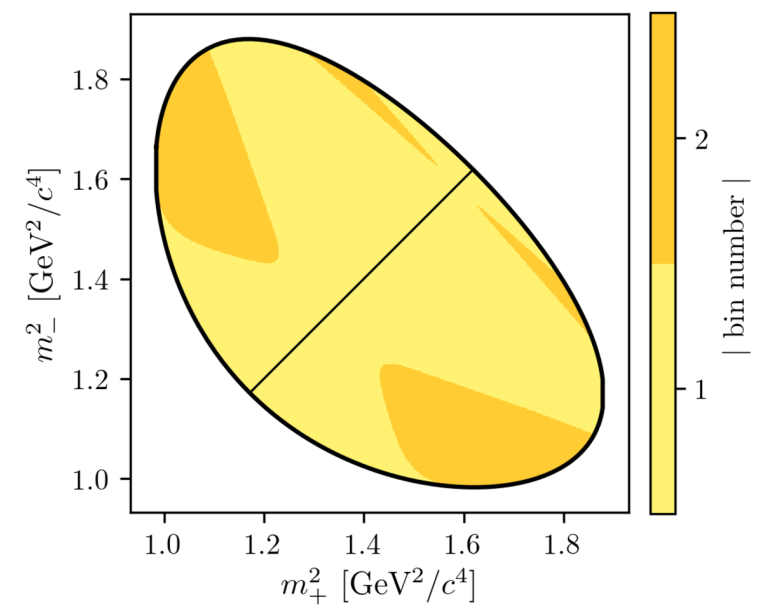
\includegraphics[width=0.5\textwidth]{KSKK2Bin.png}
  \end{figure}
  \begin{itemize}
    \item{Generated events outside phase space?}
    \item{Reconstructed events outside phase space, should I ignore?}
  \end{itemize}
\end{frame}

\begin{frame}{Bin migration}
  \begin{itemize}
    \item{Bin migration for $K_SKK$ vs $K\pi$:}
  \end{itemize}
  \vspace{0.5cm}
  \centering
  \def\arraystretch{1.2}%
  \begin{tabular}{c|cccc}
    \hline
    Generated/Reconstructed & $1$    & $2$    & $-1$   & $-2$ \\
    \hline
    $1$                     & $5233$ & $194$  & $69$   & $0$ \\
    $2$                     & $298$  & $4087$ & $0$    & $0$ \\
    $-1$                    & $68$   & $0$    & $4998$ & $215$ \\
    $-2$                    & $0$    & $0$    & $217$  & $2782$ \\
    \hline
  \end{tabular}
  \vspace{0.5cm}
  \begin{itemize}
    \item{Question: Do I need any $m_\text{BC}$ requirements when constructing this matrix?}
  \end{itemize}
\end{frame}

\begin{frame}{Sideband background subtraction method}
  \begin{figure}
    \centering
    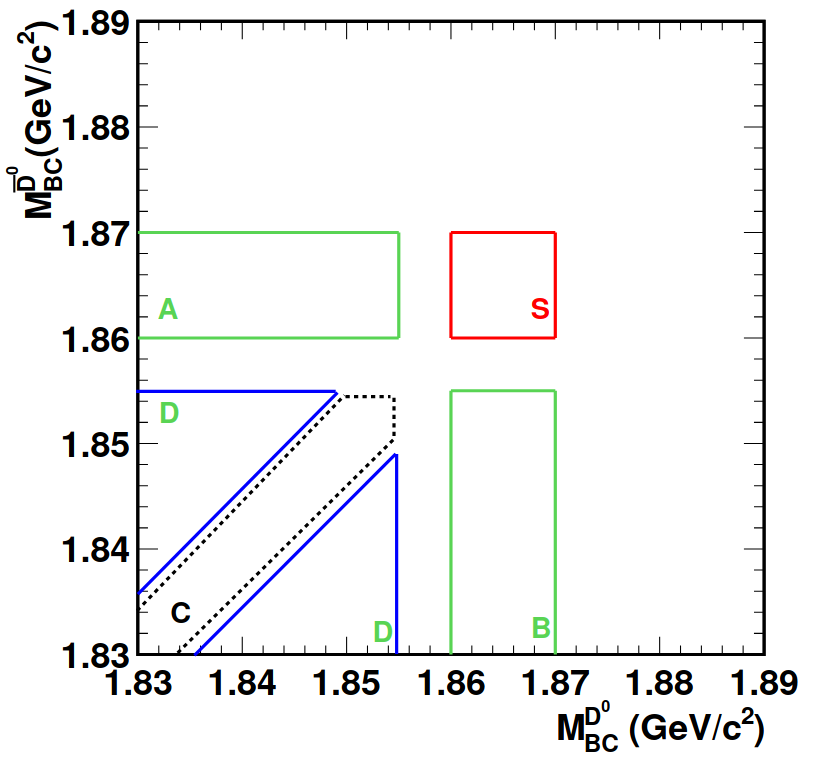
\includegraphics[width=0.45\textwidth]{MBC2D.png}
  \end{figure}
  \begin{equation*}
    B = \frac{a_S}{a_D}Y_D + \sum_{i = A, B, C}\frac{a_S}{a_i}\Big(Y_i - \frac{a_i}{a_D}Y_D\Big)
  \end{equation*}
  Question: How do I calculate errors (low number statistics)?
\end{frame}

\section{Results}
\begin{frame}{$K\pi$ double tag yield results}
  \begin{itemize}
    \item{Bin efficiency:}
    \begin{enumerate}
      \item{Count number of generated events in each bin}
      \item{Count number of truth matched events in each bin after full selection (including sideband subtraction)}
    \end{enumerate}
  \end{itemize}
  \vspace{0.5cm}
  \centering
  \def\arraystretch{1.2}%
  \begin{tabular}{l|cccc}
    \hline
    Bin & $1$    & $2$    & $-1$   & $-2$ \\
    \hline
    Yield in signal region    & $89$    & $72$    & $94$    & $69$ \\
    Sideband subtracted yield & $88.4$  & $71.4$  & $94.0$  & $69.0$ \\
    Bin migration corrected   & $89.0$  & $70.1$  & $95.2$  & $67.0$ \\
    Bin efficiency            & $9.3\%$ & $7.8\%$ & $9.7\%$ & $7.3\%$ \\
    Final double tag yield    & $0.255$ & $0.240$ & $0.261$ & $0.245$ \\
    \hline
  \end{tabular}
  \vspace{0.5cm}
  \begin{itemize}
    \item{Question: Do I use $\sqrt{N}$ for signal MC yield errors?}
  \end{itemize}
\end{frame}

\section{Results}
\begin{frame}{$K\pi\pi^0$ and $K\pi\pi\pi$ double tag yield results}
  \centering
  \def\arraystretch{1.2}%
  \begin{tabular}{l|cccc}
    \hline
    Bin & $1$    & $2$    & $-1$   & $-2$ \\
    \hline
    Bin migration corrected ($K\pi\pi^0$)  & $154.6$ & $96.4$  & $201.7$ & $131.7$ \\
    Bin efficiency ($K\pi\pi^0$)           & $3.8\%$ & $2.9\%$ & $3.7\%$ & $3.0\%$ \\
    Bin migration corrected ($K\pi\pi\pi$) & $120.6$ & $64.0$  & $139.0$ & $86.1$ \\
    Bin efficiency ($K\pi\pi\pi$)          & $7.2\%$ & $5.8\%$ & $7.2\%$ & $5.6\%$ \\
    Final double tag yield ($K_i$)         & $0.277$ & $0.161$ & $0.343$ & $0.219$ \\
    \hline
  \end{tabular}
\end{frame}

\section{Next steps}
\begin{frame}{Next steps}
  \begin{itemize}
    \setlength\itemsep{2em}
    \item{Tuple for $K_SKK$ vs $Ke\nu$ ready, combine with $K\pi\pi^0$ and $K\pi\pi\pi$}
    \item{Study peaking backgrounds in inclusive MC}
    \item{Repeat with $K_LKK$}
  \end{itemize}
\end{frame}

\end{document}
